
\chapter{Example: $\mathbf{fc}$-Multicategories}
\lbl{ch:fcm}


\chapterquote{%
A lot of people are afraid of heights.  Not me.  I'm afraid of widths.}{%
Steven Wright}


\noindent
The generalized multicategories that we are interested in typically have some
geometry to them.  They are often `higher-dimensional' in some sense.  In
this chapter we study a 2-dimensional example, \fc-multicategories, which
are $T$-multicategories when $T$ is the free category monad $\fc$ on the
category of directed graphs.

This case is interesting for a variety of reasons.  First,
\fc-multicategories turn out to encompass a wide range of familiar
2-dimensional structures, including bicategories, double categories,
monoidal categories and plain multicategories.  Second, there are two
well-known ideas for which \fc-multicategories provide a cleaner and more
general context than is traditional: the `bimodules construction' (usually
done on bicategories) and the enrichment of categories (usually done in
monoidal categories).  Third, these 2-dimensional structures are the second
rung on an infinite ladder of higher-dimensional structures (the first rung
being ordinary categories), and give us clues about the behaviour of the
more difficult, less easily visualized higher rungs.

We start~(\ref{sec:fcm}) by unwinding the definition of \fc-multicategory
to give a completely elementary description.  As mentioned above, various
familiar structures arise as special kinds of \fc-multicategory; we show
how this happens.  

A nearly-familiar structure that arises as a special kind of
\fc-multicategory is the `weak double category', in which horizontal
composition only obeys associativity and unit laws up to coherent
isomorphism.  We define these in~\ref{sec:wk-dbl} and give examples, of
which there are many natural and pleasing ones.  

Section~\ref{sec:mmm} is on the `bimodules%
%
\index{bimodules construction}
%
construction' or, as we prefer
to call it, the `monads%
%
\index{monads construction}
%
construction'.  This takes an \fc-multicategory $C$
as input and produces a new \fc-multicategory $\Mon(C)$ as output.  For
example, if $C$ is the \fc-multicategory of sets (and functions, and spans)
then $\Mon(C)$ is the \fc-multicategory of categories (and functors, and
modules); if $C$ is abelian groups (and homomorphisms) then $\Mon(C)$ is
rings (and homomorphisms, and modules).  We wait until~\ref{sec:enr-mtis}
to see what a `category enriched in an \fc-multicategory' is.




\section{$\mathbf{fc}$-multicategories}
\lbl{sec:fcm}


Let $\scat{H}$ be the category $(0 \parpair{\sigma}{\tau} 1)$ and $\Eee
= \ftrcat{\scat{H}^\op}{\Set}$.  Then $\Eee$ is the category of directed
graphs, and there is a forgetful functor $U: \Cat \go \Eee$.  This has a
left adjoint $F$: if $E \in \Eee$ then objects of $FE$ are vertices of $E$,
arrows in $FE$ are strings 
\[
x_0 \goby{p_1} x_1 \goby{p_2} \ \cdots\ \goby{p_n} x_n
\]
of edges in $E$ (with $n\geq 0$), and composition is concatenation.  The
adjunction induces a monad $T=U\of F$ on $\Eee$, which can be shown to be
cartesian either by direct calculation or by applying some general
theory~(\ref{eg:fc-cart}).  We write $T = \fc$,%
% 
\glo{fcprecise}%
%
\index{category!free (fc)@free ($\fc$)}
%
% 
for `free category', and so
we have the notion of an \fc-multicategory.

What is an \fc-multicategory,%
%
\index{fc-multicategory@$\fc$-multicategory}
%
explicitly?  An \fc-graph%
%
\index{fc-graph@$\fc$-graph}
%
$C$ is a diagram
\[
\begin{diagram}[height=2em,noPS]
	&	&C_1=(C_{11}&\pile{\rTo\\ \rTo}	&C_{10})&	&	\\
	&	&\ldTo	&			&\rdTo	&	&	\\
\fc(C_0)=(C'_{01}&\pile{\rTo\\ \rTo}&C_{00})&		&
C_0=(C_{01} &\pile{\rTo\\ \rTo}&C_{00})\\
\end{diagram}
\]
where $C_1$ and $C_0$ are directed graphs and the diagonal arrows are maps
of graphs, the $C_{ij}$'s are sets and the horizontal arrows are functions,
and $C'_{01}$ is the set of strings of edges in $C_0$.  Think of elements
of $C_{00}$ as \demph{objects} or \demph{0-cells},%
%
\index{cell!fc-multicategory@of $\fc$-multicategory}
%
elements of $C_{01}$ as
\demph{horizontal 1-cells}, elements of $C_{10}$ as \demph{vertical
1-cells}, and elements of $C_{11}$ as \demph{2-cells}, as in the picture
%
\begin{equation}	\label{diag:fcm-two-cell}
\begin{fcdiagram}
a_0	&\rTo^{m_1}	&a_1	&\rTo^{m_2}	&\ 	&\cdots	
&\ 	&\rTo^{m_n}	&a_n	\\
\dTo<{f}&		&	&		&\Downarrow\tcs{\theta}&
&	&		&\dTo>{f'}\\
a	&		&	&		&\rTo_{m}	&	
&	&		&a'	\\
\end{fcdiagram}
\end{equation}
%
($n\geq 0$, $a_i, a, a' \in C_{00}$, $m_i, m \in C_{01}$, $f, f' \in C_{10}$,
$\theta\in C_{11}$).  An \fc-multicategory
structure on the \fc-graph $C$
amounts to composition and identities of two types.  First, the directed
graph 
\[
\begin{slopeydiag}
	&	&C_{10}	&	&	\\
	&\ldTo	&	&\rdTo	&	\\
C_{00}	&	&	&	&C_{00}	\\
\end{slopeydiag}
\]
has the structure of a category; in other words, vertical 1-cells can be
composed and there is an identity vertical 1-cell on each 0-cell.  Second,
there is a composition function for 2-cells,
%
\begin{equation}	\label{eq:pasted-two-cells}
\begin{array}{l}
\begin{diagram}[width=.5em,height=2em]
\blob&\rTo^{m_1^1}&\cdots&\rTo^{m_1^{k_1}}&
\blob&\rTo^{m_2^1}&\cdots&\rTo^{m_2^{k_2}}&\blob&
\ &\cdots&\ &
\blob&\rTo^{m_n^1}&\cdots&\rTo^{m_n^{k_n}}&\blob\\
\dTo<{f_0}&&\Downarrow\tcs{\theta_1}&&
\dTo<{f_1}&&\Downarrow\tcs{\theta_2}&&\dTo&
\ &\cdots&\ &
\dTo&&\Downarrow\tcs{\theta_n}&&\dTo>{f_n}\\
\blob&&\rTo_{m_1}&&
\blob&&\rTo_{m_2}&&\blob&
\ &\cdots&\ &
\blob&&\rTo_{m_n}&&\blob\\
\dTo<{f}&&&&&&&\Downarrow\tcs{\theta} &&&&&&&&&\dTo>{f'}\\
\blob&&&&&&&&\rTo_{m}&&&&&&&&\blob\\
\end{diagram}
\\
\\
\goesto\diagspace
% 
\begin{diagram}[width=.5em,height=2em]
\blob&\rTo^{m_1^1}&\ &&
&&&&\cdots&
&&&
&&\ &\rTo^{m_n^{k_n}}&\blob\\
\dTo<{f\of f_0}&&&&&&&&
\Downarrow\tcs{\theta\of\tuple{\theta_1}{\theta_2}{\theta_n}}
&&&&&&&&\dTo>{f'\of f_n}\\
\blob&&&&&&&&\rTo_{m}&&&&&&&&\blob\\
\end{diagram}
\end{array}
\end{equation}
% 
($n\geq 0, k_i\geq 0$, with \blob's representing objects), and a function
assigning an identity 2-cell to each horizontal 1-cell,
\[
\begin{fcdiagram}
a&\rTo^{m}&a'\\
\end{fcdiagram}
\diagspace\goesto\diagspace
\begin{fcdiagram}
a&\rTo^{m}&a'\\
\dTo<{1_a}&\Downarrow \tcs{1_m}&\dTo>{1_{a'}}\\
a&\rTo_{m}&a'.\\
\end{fcdiagram}
\]
The composition and identities obey associativity and identity laws, which
ensure that any diagram of pasted-together 2-cells with a rectangular
boundary has a well-defined composite.

The pictures in the nullary%
%
\index{nullary!composite}%
%
\index{fc-multicategory@$\fc$-multicategory!nullary composite in}
%
case are worth a short comment.
When $n=0$, the 2-cell of diagram~\bref{diag:fcm-two-cell} is drawn as
\[
\begin{fcdiagram}
a_0		&\rEquals		&a_0		\\
\dTo<{f}	&\Downarrow\tcs{\theta}	&\dTo>{f'}	\\
a		&\rTo_{m}		&a',		\\
\end{fcdiagram}
\]
and the diagram of pasted-together 2-cells in the domain
of~\bref{eq:pasted-two-cells} is drawn as
\[
\begin{fcdiagram}
b_0		&\rEquals		&b_0		\\
\dTo<{f_0}	&=			&\dTo>{f_0}	\\
a_0		&\rEquals		&a_0		\\
\dTo<{f}	&\Downarrow\tcs{\theta}	&\dTo>{f'}	\\
a		&\rTo_{m}		&a'.		\\
\end{fcdiagram}
\]
The composite%
\lbl{p:null-notation}
of this last diagram will be written as $\theta\of f_0$.

So in completely elementary terms, an \fc-multicategory consists of
%
\begin{itemize}
\item a set of objects
\item for each pair $(a,a')$ of objects, a set of vertical 1-cells 
$
\begin{fcdiagram}
a	\\
\dTo	\\
a'	\\
\end{fcdiagram}
$
\item for each pair $(a,a')$ of objects, a set of horizontal 1-cells
$a \go a'$
\item for each $a_0, \ldots, a_n, a, a', m_1, \ldots, m_n, m, f, f'$ as
in~\bref{diag:fcm-two-cell}, a set of 2-cells $\theta$
\item composition and identity functions for vertical 1-cells, as described
above
\item composition and identity functions for 2-cells, as described above,
\end{itemize}
%
satisfying associativity and identity axioms.  Having given this elementary
description I will feel free to refer to large \fc-multicategories, in
which the collection of cells is a proper class.

\begin{example}	\lbl{eg:fcm-Ring}
There is an \fc-multicategory \fcat{Ring}%
% 
\glo{fcRing}%
%
\index{fc-multicategory@$\fc$-multicategory!rings@of rings}
%
% 
in which
%
\begin{itemize}
\item 0-cells are (not necessarily commutative) rings
\item vertical 1-cells are ring homomorphisms
\item a horizontal 1-cell $A \go A'$ is an
  $(A',A)$-bimodule~(\ref{eg:bicat-Ring})%
%
\index{module!bimodule over rings}
%

\item a 2-cell  
\[
\begin{fcdiagram}
A_0	&\rTo^{M_1}	&A_1	&\rTo^{M_2}	&\ 	&\cdots	
&\ 	&\rTo^{M_n}	&A_n	\\
\dTo<{f}&		&	&		&\Downarrow\tcs{\theta}&
&	&		&\dTo>{f'}\\
A	&		&	&		&\rTo_{M}	&	
&	&		&A'	\\
\end{fcdiagram}
\]
is an abelian group homomorphism
\[
\theta: 
M_n \otimes_{A_{n-1}} M_{n-1} \otimes_{A_{n-2}} \cdots
\otimes_{A_1} M_1
\go 
M
\]
satisfying
\[
\theta(a_n\cdot m_n \otimes m_{n-1} \otimes\cdots\otimes
m_2 \otimes m_1\cdot a_1)
=
f'(a_n) \cdot 
\theta(m_n \otimes\cdots\otimes m_1)
\cdot f(a_1)
\]
(that is, $\theta$ is a homomorphism of $(A_n, A_0)$-bimodules if $M$ is
given an $(A_n, A_0)$-bimodule structure via $f$ and $f'$)
\item composition and identities are defined in the evident way.
\end{itemize}
%
Thus, rings, homomorphisms of rings, modules over rings, homomorphisms of
modules, and tensor products of modules are integrated into a single
structure.  The category formed by the objects and vertical 1-cells is the
ordinary category of rings and homomorphisms.  When the distinction needs
making, I will write $\fcat{Ring}_1$ for this `1-dimensional' category and
$\fcat{Ring}_2$%
% 
\glo{fcRing2}
% 
for the `2-dimensional' \fc-multicategory.  Similar
notation is extended to similar examples.
\end{example}

Many familiar 2-dimensional%
%
\index{algebraic theory!two-dimensional@2-dimensional}
% 
structures are degenerate \fc-multicategories.
The following examples demonstrate this; Fig.~\ref{fig:degens} is a
summary.
%
\begin{figure}\protect\small
\begin{tabular}{llll}	
			&\emph{No horizontal}	&\emph{Weak horizontal}	&
\emph{Strict horizontal}\\
			&\emph{composition}	&\emph{composition}	&
\emph{composition}	\\
\\
\emph{No degeneracy}	&\fc-multicategory	&Weak double		&
Strict double		\\
			&			&category		&
category		\\
\\
\emph{All vertical 1-cells}&Vertically discrete	&Bicategory		&
Strict			\\
\emph{are identities}	&\fc-multicategory	&			&
2-category		\\
\\
\emph{Only one object and}&Plain		&Monoidal		&
Strict monoidal \\
\emph{one vertical 1-cell}&multicategory	&category		&
category
\end{tabular}%
%
\index{fc-multicategory@$\fc$-multicategory!degenerate}
% 
\caption{Some of the possible degeneracies of an \fc-multicategory. The
left-hand column refers to degeneracies in the category formed by the
objects and vertical 1-cells. The top row says whether the
\fc-multicategory structure arises from a composition rule for horizontal
1-cells. See Examples~\ref{eg:fcm-str-dbl}--\ref{eg:fcm-mon-cat}}
\label{fig:degens}
\end{figure}

\begin{example}	\lbl{eg:fcm-str-dbl}%
%
\index{double category!strict!fc-multicategory@as $\fc$-multicategory}%
%
\index{fc-multicategory@$\fc$-multicategory!strict double category@from strict double category}
%
Any strict double category gives rise to an \fc-multicategory, in which a
2-cell as in~\bref{diag:fcm-two-cell} is a 2-cell
%
\begin{diagram}[height=2em]
a_0	&\rTo^{m_n \of \cdots \of m_1}	&a_n\\
\dTo<{f}&\Downarrow\tcs{\theta}		&\dTo>{f'}\\
a	&\rTo_{m}			&a'\\
\end{diagram}
%
in the double category.
\end{example}

\begin{example}	\lbl{eg:fcm-wk-dbl}
The last example works just as well if we start with a double category in
which the composition of horizontal 1-cells only obeys weak laws.  We call
these `weak%
%
\index{fc-multicategory@$\fc$-multicategory!weak double category@from weak double category}%
%
\index{double category!weak!fc-multicategory@as $\fc$-multicategory}
%
double categories' and discuss them in detail in the next
section; a typical example is \fcat{Ring}~(\ref{eg:fcm-Ring}).  A similar
example, and really the archetypal weak double category, is $\Set_2$,%
% 
\glo{fcSet2}%
%
\index{fc-multicategory@$\fc$-multicategory!sets@of sets}
%
% 
defined as follows:
%
\begin{itemize}
\item objects are sets
\item vertical 1-cells are functions (and the category formed by objects
and vertical 1-cells is the ordinary category $\Set_1$ of sets and
functions; see~\ref{eg:fcm-Ring} for the notation)
\item horizontal 1-cells are spans:%
%
\index{span}
%
that is, a horizontal 1-cell $A \go A'$
is a diagram
\[
\begin{slopeydiag}
	&	&M	&	&	\\
	&\ldTo	&	&\rdTo	&	\\
A	&	&	&	&A'	\\
\end{slopeydiag}
\]
of sets and functions
\item a 2-cell inside
\[
\begin{slopeydiag}
	&	&M	&	&	\\
	&\ldTo	&	&\rdTo	&	\\
A	&	&	&	&A'	\\
\dTo<f	&	&N	&	&\dTo>{f'}\\
	&\ldTo	&	&\rdTo	&	\\
B	&	&	&	&B'	\\
\end{slopeydiag}
\]
is a function $\theta: M \go N$ making the diagram commute
\item horizontal composition is by pullback.
\end{itemize}
%
That every weak double category has an underlying \fc-multicategory is
exactly analogous to every weak monoidal category having an underlying
plain multicategory.
\end{example}

\begin{example}	\lbl{eg:fcm-vdisc}
Consider $\fc$-multicategories $C$ in which all vertical 1-cells are
identities.  This means that the category formed by the objects and
vertical 1-cells is discrete, so we call $C$ \demph{vertically discrete}.%
%
\index{fc-multicategory@$\fc$-multicategory!vertically discrete}
%
A vertically discrete \fc-multicategory consists of some objects $a, a',
\ldots$, some 1-cells $m, m',\ldots$, and some 2-cells looking like
%
\begin{equation}	\label{diag:fc-ope-two-cell}
\begin{diagram}[size=1.5em,tight,scriptlabels]
		&	&	&a_2	&\ldots	&	&	&	\\
		&a_1	&\ruEdge(2,1)^{m_2}&&	&	&a_{n-1}&	\\
\ruEdge(1,2)<{m_1}&	&	&	&\Downarrow \tcs{\theta}&&
&\rdEdge(1,2)>{m_{n}}							\\
a_0		&	&	&\rEdge_{m}&	&	&	&a_n,	\\
\end{diagram}
\end{equation}
%
together with a composition function
% 
\[
\begin{array}{c}
\setlength{\unitlength}{1mm}
\begin{picture}(49,25)(0,-2)
\cell{0}{0}{bl}{
\includegraphics{vdcompdom.eps}}
% 0-cell labels
\cell{10}{1.5}{t}{a_0}
\cell{15.5}{15.5}{t}{a_1}
\cell{35}{15.5}{t}{a_{n-1}}
\cell{40}{1.5}{t}{a_n}
% 1-cell labels
\cell{25}{0}{t}{\scriptstyle m}
\cell{15}{8}{c}{\scriptstyle m_1}
\cell{34.5}{8}{c}{\scriptstyle m_n}
\cell{5}{2}{c}{\scriptstyle m_1^1}
\cell{10}{17.5}{c}{\scriptstyle m_1^{k_1}}
\cell{39}{17.5}{c}{\scriptstyle m_n^1}
\cell{46.5}{4}{c}{\scriptstyle m_n^{k_n}}
% 2-cell labels
\cell{25}{7}{c}{\Downarrow\theta}
% 
\da{8}{8}{68}
\cell{9}{11}{c}{\theta_1}
% 
\da{42}{8}{-68}
\cell{41}{11}{c}{\theta_n}
\end{picture}
\end{array}
%
\ \goesto \ 
% 
\begin{array}{c}
\setlength{\unitlength}{1mm}
\begin{picture}(49,25)(0,-2)
\cell{0}{0}{bl}{
\includegraphics{vdcompcod.eps}}
% 0-cell labels
\cell{10}{1.5}{t}{a_0}
\cell{40}{1.5}{t}{a_n}
% 1-cell labels
\cell{25}{0}{t}{\scriptstyle m}
\cell{5}{2}{c}{\scriptstyle m_1^1}
\cell{46.5}{4}{c}{\scriptstyle m_n^{k_n}}
% 2-cell labels
\cell{25}{7}{c}{\Downarrow \theta \of (\theta_1, \ldots, \theta_n)}
\end{picture}
\end{array}
\]
and an identity function
\[
\begin{array}{c}
\setlength{\unitlength}{1mm}
\begin{picture}(33,5)
\cell{3}{2}{l}{\includegraphics{vdiddom.eps}}
\cell{2.5}{1.3}{br}{a}
\cell{30}{1.3}{bl}{a'}
\cell{16}{3}{b}{\scriptstyle m}
\end{picture}
\end{array}
%
\diagspace\goesto\diagspace
% 
\begin{array}{c}
\setlength{\unitlength}{1mm}
\begin{picture}(33,13)(0,1)
\cell{3}{3}{bl}{
\includegraphics{vdidcod.eps}}
\cell{2.5}{3.5}{br}{a}
\cell{30}{3.5}{bl}{a'}
\cell{16}{2.5}{t}{\scriptstyle m}
\cell{16}{12.5}{b}{\scriptstyle m}
\cell{16}{7}{c}{\Downarrow 1_m}
\end{picture}
\end{array}
\]
obeying the inevitable associativity and identity laws.  This leads us into
the world of opetopes%
%
\index{opetope}
%
(Chapter~\ref{ch:opetopic}).
\end{example}

\begin{example}	\lbl{eg:fcm-bicat}
A bicategory%
%
\index{bicategory!fc-multicategory@as $\fc$-multicategory}%
%
\index{fc-multicategory@$\fc$-multicategory!bicategory@from bicategory}
%
%
is a weak double category in which the only vertical 1-cells
are identities, and so gives rise to an \fc-multicategory.  Explicitly, if
$B$ is a bicategory then there is a vertically discrete $\fc$-multicategory
whose objects are those of $B$, whose horizontal 1-cells are the 1-cells of
$B$, and whose 2-cells~\bref{diag:fc-ope-two-cell} are 2-cells
\[
a_0 
\ctwomult{\scriptstyle (m_n \sof\cdots\sof m_1)}%
{\scriptstyle m}{\tcs{\theta}} 
a_n
\]
in $B$.
\end{example}

\begin{example}	\lbl{eg:fcm-cl-mti}%
%
\index{multicategory!fc-multicategory@as $\fc$-multicategory}%
%
\index{fc-multicategory@$\fc$-multicategory!plain multicategory@from plain multicategory}
%
Plain multicategories are the same as \fc-multicategories with only
one object and one vertical 1-cell.  If the plain multicategory is
called $M$ then we call the corresponding \fc-multicategory $\Sigma M$,%
% 
\glo{Sigmamtifc}
% 
the \demph{suspension}%
%
\index{suspension!plain multicategory@of plain multicategory}%
%
\index{multicategory!suspension of}
%
%
of $M$.  Horizontal 1-cells in $\Sigma M$ are objects
of $M$, and 2-cells
%
\begin{equation}	\label{diag:fcm-cl-mti-cell}
\begin{diagram}[size=1.5em,tight,abut]
		&	&	&\	&\ldots	&	&	&	\\
		&\bullet&\ruTo(2,1)^{m_2}&&	&	&\	&	\\
\ruTo(1,2)<{m_1}&	&	&	&\Downarrow \tcs{\theta}&&	
&\rdTo(1,2)>{m_n}							\\
\bullet		&	&	&\rTo_{m}&	&	&	&\bullet\\
\end{diagram}
\end{equation}
%
in $\Sigma M$ are maps
\[
m_1, \ldots, m_n \goby{\theta} m
\]
in $M$.
\end{example}

\begin{example}	\lbl{eg:fcm-cl-opd}
In particular, plain operads are \fc-multicategories in which there is only
one object, one vertical 1-cell and one horizontal 1-cell.  An \fc-operad%
%
\index{fc-operad@$\fc$-operad}
%
is an \fc-multicategory in which there is only one object and one
horizontal 1-cell, so a plain operad is a special kind of \fc-operad.

If we are going to take the suspension%
%
\index{suspension!plain operad@of plain operad}%
%
\index{operad!suspension of}
%
%
idea seriously then we should write
\[
\Sigma: \Operad \rIncl \Multicat
\]
for the inclusion of operads as one-object multicategories.  We also
have~(\ref{eg:fcm-cl-mti}) the suspension map
\[
\Sigma: \Multicat \rIncl \fc\hyph\Multicat,
\]
so the inclusion of operads into \fc-multicategories should be written
$\Sigma^2$: double suspension.  Of course, we usually leave the first
inclusion nameless.
\end{example}

\begin{example}	\lbl{eg:fcm-mon-cat}
As a special case of both~\ref{eg:fcm-bicat} and~\ref{eg:fcm-cl-mti}, any
monoidal%
%
\index{monoidal category!fc-multicategory@as $\fc$-multicategory}%
%
\index{fc-multicategory@$\fc$-multicategory!monoidal category@from monoidal category}
%
category $M$ gives rise to an \fc-multicategory $\Sigma M$ in
which there is one object and one vertical 1-cell.  Horizontal 1-cells are
objects of $M$, and 2-cells~\bref{diag:fcm-cl-mti-cell} are maps 
\[
\theta: (m_n \otimes\cdots\otimes m_1) \go m
\]
in $M$.  
\end{example}

\begin{example}	\lbl{eg:fcm-matrices}
Here is a family of \fc-multicategories that are not usually degenerate%
%
\index{fc-multicategory@$\fc$-multicategory!non-degenerate}
%
in
any of the ways listed above.  Let $V$ be a plain multicategory and define
the \fc-multicategory $\Set[V]$ as follows:
%
\begin{itemize}
\item objects are sets
\item vertical 1-cells are functions
\item a horizontal 1-cell $A \go A'$ is a family $(m_{a,a'})_{a\in A, a'\in
A'}$ of objects of $V$
\item a 2-cell
\[
\begin{fcdiagram}
A_0	&\rTo^{m^1}	&A_1	&\rTo^{m^2}	&\ 	&\cdots	
&\ 	&\rTo^{m^n}	&A_n	\\
\dTo<{f}&		&	&		&\Downarrow\tcs{\theta}&
&	&		&\dTo>{f'}\\
A	&		&	&		&\rTo_{m}	&	
&	&		&A'	\\
\end{fcdiagram}
\]
is a family
\[
\left(
m^1_{a_0, a_1}, \ldots, m^n_{a_{n-1}, a_n}
\goby{\theta_{a_0, \ldots, a_n}}
m_{f(a_0), f'(a_n)}
\right)_{a_0 \in A_0, \ldots, a_n \in A_n}
\]
of maps in $V$
\item composition and identities are obvious. 
\end{itemize}
%
If $V=\Set$ then $\Set[V]$ is the \fc-multicategory $\Set_2$
of~\ref{eg:fcm-wk-dbl}.  But $\Set[V]$ is not (the underlying
\fc-multicategory of) a weak double category unless $V$ happens to be (the
underlying plain multicategory of) a monoidal category, since $\Set[V]$
does not usually have `enough universal 2-cells'.  Compare the results on
representable%
%
\index{fc-multicategory@$\fc$-multicategory!representable}
%
multicategories in~\ref{sec:non-alg-notions}.
\end{example}

We will not be much concerned with algebras%
%
\index{algebra!for fc-multicategory@for $\fc$-multicategory}%
%
\index{fc-multicategory@$\fc$-multicategory!algebra for}
%
%
for \fc-multicategories, but
let us look at them briefly.  Given an object $E$ of $\Eee$, that is, a
directed graph, an object $(X\go E)$ of $\Eee/E$ amounts to a set $X(a)$
for each vertex $a$ of $E$ and a span 
\[
\begin{slopeydiag}
	&	&X(m)	&	&	\\
	&\ldTo	&	&\rdTo	&	\\
X(a)	&	&	&	&X(b)	\\
\end{slopeydiag}
\]
for each edge $a \goby{m} b$ of $E$.  An algebra for an \fc-multicategory
$C$ is an object $(X \go C_0)$ of $\Eee/C_0$ together with an action of $C$
on $X$, and so a $C$-algebra is just an \fc-multicategory map from $C$ into
the (large) \fc-multicategory $\Set_2$ defined in~\ref{eg:fcm-wk-dbl}.

There are some interesting examples of algebras when $C$ is the
\fc-multicategory coming from a plain operad $P$: in the notation
of~\ref{eg:fcm-cl-opd}, $C = \Sigma P$.  A $(\Sigma P)$-algebra is called a
\demph{categorical $P$-algebra}%
%
\index{categorical algebra for operad}%
%
or a \demph{$P$-category},%
%
\lbl{p:P-category}%
%
\index{operad!category over}
%
and consists of a directed graph $X$ together with a function
%
\begin{equation}	\label{eq:P-cat-action}
P(n) \times X(x_{n-1}, x_n) \times \cdots \times X(x_0, x_1)
\go
X(x_0, x_n)
\end{equation}
%
for each $n\in\nat$ and sequence $x_0, \ldots, x_n$ of vertices of $X$,
satisfying the evident axioms.  (Here $X(x,x')$ denotes the set of edges
from $x$ to $x'$.)  If $P=1$ then a $P$-category is exactly a category;
there are some less trivial examples too.

\begin{example}	\lbl{eg:fc-Trimble}%
%
\index{operad!path reparametrizations@of path reparametrizations}
%
Let $E$ be the operad in which 
\[
E(n) =
\{
\textrm{endpoint-preserving continuous maps }
[0,1] \go [0,n]
\},
\]
as in~\ref{eg:opd-Trimble}, so that any loop space is naturally an
$E$-algebra.  Then any path-space is naturally an $E$-category.  In other
words, take a topological space $Y$ and let $X$ be the graph whose vertices
are points of $Y$ and whose edges are continuous maps from $[0,1]$ into
$Y$: then $X$ is naturally a $E$-category.  
\end{example}

\begin{example}	\lbl{eg:fc-A-infty}%
%
\index{A-@$A_\infty$-!algebra}%
%
\index{A-@$A_\infty$-!category}
%
Similarly, taking $A_\infty$ to be the operad of chain complexes whose
algebras are $A_\infty$-algebras (p.~\pageref{p:A-infty-alg}) gives us the
standard notion of an \demph{$A_\infty$-category}.  For this to make sense,
we must work in a world where everything is enriched in chain complexes: so
$X$ consists of a set $X_0$ of objects (or vertices) together with a chain
complex $X(x,x')$ for each pair $(x,x')$ of objects, and
in~\bref{eq:P-cat-action} the $\times$'s become $\otimes$'s.  We do not
meet enriched generalized multicategories properly
until~\ref{sec:enr-mtis}, but it is clear how things should work in this
particular situation.
\end{example}




\section{Weak double categories}
\lbl{sec:wk-dbl}

Generalizing both bicategories and strict double categories are `weak
double categories', introduced informally in~\ref{sec:fcm}.  Recall that
these are only weak in the horizontal direction: vertical composition still
obeys strict laws.  We do not consider double categories weak in both
directions.

The definition of weak double category is a cross between that of strict
double category and that of unbiased bicategory.
% 
\begin{defn}%
%
\index{double category!weak}
%
A \demph{weak double category} $D$ consists of some data subject
to some axioms.  The data is:
%
\begin{itemize}
\item A diagram
\[
\begin{slopeydiag}
	&	&D_1	&	&	\\
	&\ldTo<\dom&	&\rdTo>\cod&	\\
D_0	&	&	&	&D_0	\\
\end{slopeydiag}
\]
of categories and functors.  The objects of $D_0$ are called the
\demph{0-cells}%
%
\index{cell!weak double category@of weak double category}
%
or \demph{objects} of $D$, the maps in $D_0$ are the
\demph{vertical 1-cells} of $D$, the objects of $D_1$ are the
\demph{horizontal 1-cells} of $D$, and the maps in $D_1$ are the
\demph{2-cells} of $D$, as in the picture
%
\begin{equation}	\label{diag:wk-dbl-two-cell}
\begin{fcdiagram}
a	&\rTo^m			&a'	\\
\dTo<f	&\Downarrow\tcs{\theta}	&\dTo>{f'}\\
b	&\rTo_p			&b'	\\
\end{fcdiagram}
\end{equation}
%
where $a \goby{f} b$, $a' \goby{f'} b'$ are maps in $D_0$ and $m
\goby{\theta} p$ is a map in $D_1$, with $\dom(m) = a$, $\dom(\theta)=f$,
and so on. 
\item For each $n\geq 0$, a functor $\comp^{(n)}: D_1^{(n)} \go D_1$ such
that the diagram
\[
\begin{slopeydiag}
	&	&D_1^{(n)}		&	&	\\
	&\ldTo	&			&\rdTo	&	\\
D_0	&	&\dTo~{\comp^{(n)}}	&	&D_0	\\
	&\luTo<\dom&			&\ruTo>\cod&	\\
	&	&D_1			&	&	\\
\end{slopeydiag}
\]
commutes, where $D_1^{(n)}$ is the limit of the diagram
\[
\begin{slopeydiag}
	&	&D_1	&	&	&	&D_1	&	&
	&	&	&	&D_1	&	&	\\
	&\ldTo<\dom&	&\rdTo>\cod&	&\ldTo<\dom&	&\rdTo>\cod&
	&	&	&\ldTo<\dom&	&\rdTo>\cod&	\\
D_0	&	&	&	&D_0	&	&	&	&
\ 	&\cdots	&\ 	&	&	&	&D_0	\\
\end{slopeydiag}
\]
containing $n$ copies of $D_1$.  The functor $\comp^{(n)}$ is called
\demph{$n$-fold horizontal composition}%
%
\index{n-fold@$n$-fold!horizontal composition}
%
and written
\[
\begin{array}{rl}
&
\begin{fcdiagram}
a_0		&\rTo^{m_1}		&a_1		&\rTo^{m_2}	&
\cdots 	&\rTo^{m_n}		&a_n	\\
\dTo<{f_0}	&\Downarrow\tcs{\theta_1}&\dTo<{f_1}	&\Downarrow\tcs{\theta_2}&
	&\Downarrow\tcs{\theta_n}	&\dTo>{f_n}\\
b_0		&\rTo_{p_1}		&b_1		&\rTo_{p_2}	&
\cdots 	&\rTo_{p_n}		&b_n	\\
\end{fcdiagram}
\\
\\
\goesto	&
\begin{fcdiagram}
a_0 		&\rTo^{(m_n \of\cdots\of m_1)} 	&a_n	\\
\dTo<{f_0}	&\Downarrow\tcs{(\theta_n * \cdots * \theta_1)}&\dTo>{f_n}\\
b_0 		&\rTo_{(p_n \of\cdots\of p_1)} 	&b_n.	\\
\end{fcdiagram}
\end{array}
\]
\item For each double sequence 
\[
\mathbf{m} = 
((m_1^1, \ldots, m_1^{k_1}), \ldots, (m_n^1, \ldots, m_n^{k_n}))
\]
of horizontal 1-cells such that the composites below make sense, an
invertible 2-cell 
\[
\begin{fcdiagram}
\blob	&\rTo^{((m_n^{k_n} \of\cdots\of m_n^1) \of\cdots\of (m_1^{k_1}
\of\cdots\of m_1^1))}	&\blob	\\
\dTo<1	&\Downarrow \tcs{\gamma_{\mathbf{m}}}	&\dTo>1	\\
\blob 	&\rTo_{(m_n^{k_n} \of\cdots\of m_1^1)}	&\blob	\\
\end{fcdiagram}
\]
(where `invertible' refers to vertical composition).
\item For each horizontal 1-cell $a \goby{m} a'$, an invertible 2-cell
\[
\begin{fcdiagram}
a	&\rTo^m			&a'	\\
\dTo<1	&\Downarrow \tcs{\iota_m}	&\dTo>1	\\
a	&\rTo_{(m)}		&a'.	\\	
\end{fcdiagram}
\]
\end{itemize}
%
The axioms are:
%
\begin{itemize}
\item $\gamma_{\mathbf{m}}$ is natural in each of the $m_i^j$'s, and
$\iota_m$ is natural in $m$.  In the case of $\iota$, this means that for
each 2-cell $\theta$ as in~\bref{diag:wk-dbl-two-cell} we have
\[
\begin{fcdiagram}
a	&\rTo^m			&a'	\\
\dTo<f	&\Downarrow\tcs{\theta}	&\dTo>{f'}\\
b	&\rTo^p			&b'	\\
\dTo<1	&\Downarrow\tcs{\iota_p}&\dTo>1	\\
b	&\rTo_{(p)}		&b'	\\
\end{fcdiagram}
\diagspace
=
\diagspace
\begin{fcdiagram}
a	&\rTo^m			&a'	\\
\dTo<1	&\Downarrow\tcs{\iota_m}	&\dTo>1\\
a	&\rTo^{(m)}		&a'	\\
\dTo<f	&\Downarrow\tcs{(\theta)}	&\dTo>{f'}\\
b	&\rTo_{(p)}		&b',	\\
\end{fcdiagram}
\]
and similarly for $\gamma$.  
\item $\gamma$ and $\iota$ satisfy associativity and identity coherence
axioms analogous to those in the definition~(\ref{defn:lax-mon-cat}) of
lax monoidal category.  
\end{itemize}
\end{defn}

It is clear how to define lax maps between weak double categories, again
working by analogy with unbiased monoidal categories or unbiased
bicategories, and there is a forgetful functor
\[
(\textrm{weak double categories and lax maps})
\go
\fc\hyph\Multicat.
\]

\begin{example}	\lbl{eg:wk-dbl-degen}%
%
\index{double category!weak!degenerate}
%
There are several degenerate cases.  A weak double category in which the
coherence cells $\gamma$ and $\iota$ are all identities is exactly a strict
double category.  A weak double category whose only vertical 1-cells are
identities is exactly an (unbiased) bicategory.  A weak double category
whose only horizontal 1-cells are identities is exactly a strict
2-category. 
\end{example}

\begin{example}
The \fc-multicategory $\fcat{Ring}_2$%
%
\index{double category!weak!rings@of rings}
%
of~\ref{eg:fcm-Ring} is a weak double
category, horizontal composition being tensor of modules.
\end{example}

\begin{example}	\lbl{eg:wk-dbl-T-span}
The \fc-multicategory $\Set_2$%
%
\index{double category!weak!sets@of sets}
%
of~\ref{eg:fcm-wk-dbl} is also a weak double
category.  It is formed from sets, functions, and spans,%
%
\index{span}
%
which is
reminiscent of the definition of $T$-multicategories and maps between them
in~\ref{sec:om}.  Indeed, let $T$ be a cartesian monad on a cartesian
category $\Eee$, and define a weak double category as follows:
%
\begin{itemize}
\item objects are objects of $\Eee$
\item vertical 1-cells are maps in $\Eee$
\item horizontal 1-cells $E \go E'$ are diagrams
\[
\begin{slopeydiag}
	&	&M	&	&	\\
	&\ldTo<d&	&\rdTo>c&	\\
TE	&	&	&	&E'	\\
\end{slopeydiag}
\]
in $\Eee$
\item 2-cells $\theta$ are commutative diagrams
\[
\begin{slopeydiag}
	&	&L	&	&	\\
	&\ldTo	&	&\rdTo	&	\\
TD	&	&\dTo>\theta&	&D'	\\
\dTo<{Tf}&	&M	&	&\dTo>{f'}\\
	&\ldTo	&	&\rdTo	&	\\
TE	&	&	&	&E'	\\
\end{slopeydiag}
\]
\item vertical composition is as in $\Eee$
\item horizontal composition is by pullback: the composite of horizontal
1-cells
\[
\begin{slopeydiag}
	&	&M_1	&	&	\\
	&\ldTo	&	&\rdTo	&	\\
TE_0	&	&	&	&E_1,	\\
\end{slopeydiag}
\diagspace
\begin{slopeydiag}
	&	&M_2	&	&	\\
	&\ldTo	&	&\rdTo	&	\\
TE_1	&	&	&	&E_2,	\\
\end{slopeydiag}
\diagspace \ldots, \diagspace 
\begin{slopeydiag}
	&	&M_n	&	&	\\
	&\ldTo	&	&\rdTo	&	\\
TE_{n-1}&	&	&	&E_n	\\
\end{slopeydiag}
\]
is the limit of the diagram
\[
\begin{slopeydiag}
&&	&	&T^{n-1}M_1&	&	&	&T^{n-2}M_2&	&
	&	&	&	&M_n	&	&	\\
&&	&\ldTo	&	&\rdTo	&	&\ldTo	&	&\rdTo	&
	&	&	&\ldTo	&	&\rdTo	&	\\
&&T^n E_0&	&	&	&T^{n-1} E_1&	&	&	&
\ 	&\cdots	&\ 	&	&	&	&E_n	\\
&\ldTo<{\mu^{(n)}_{E_0}}&&&&	&	&	&	&	&
	&	&	&	&	&	&	\\
TE_0	&	&	&	&	&	&	&	&
	&	&	&	&	&	&	\\
\end{slopeydiag}
\]
where $\mu^{(n)}$ is the $n$-fold multiplication of the monad $T$; 
horizontal composition of 2-cells works similarly.
\end{itemize}
%
Any weak double category%
%
\index{double category!weak!bicategory@\vs.\ bicategory}%
%
\index{bicategory!weak double category@\vs.\ weak double category}
%
%
yields a bicategory by discarding all the vertical
1-cells except for the identities, and applying this to the weak double
category just defined yields the bicategory $\Sp{\Eee}{T}$
(Definition~\ref{defn:T-spans}).  It is therefore reasonable to call our
weak double category $\Sp{\Eee}{T}$%
% 
\glo{Spwkdbl}
% 
too.  In particular, $\Sp{\Set}{\id} =
\Set_2$.
\end{example}

\begin{example}	\lbl{eg:wk-dbl-Cat}
Categories, functors and modules%
%
\index{module!categories@over categories}
%
are integrated in the following weak
double category $\Cat_2$:%
% 
\glo{wkdblCat2}%
%
\index{double category!weak!categories@of categories}%
%
\index{category!weak double category of}
%
\begin{itemize}
\item objects are small categories
\item vertical 1-cells are functors
\item horizontal 1-cells are modules~(\ref{sec:om-further}): that is, a
horizontal 1-cell $A \go A'$ is a functor $A^\op \times A' \go \Set$
\item a 2-cell
\[
\begin{fcdiagram}
A	&\rTo^M		&A'	\\
\dTo<F	&\Downarrow	&\dTo>{F'}\\
B	&\rTo_P		&B'	\\
\end{fcdiagram}
\]
is a natural transformation
\[
\begin{diagram}[height=1.2em]
A^\op \times A'		&		&	&	\\
			&\rdTo(3,2)>M	&	&	\\
\dTo<{F\times F'}	&\sent		&	&\Set	\\
			&		&\ruTo(3,2)>P	&	\\
B^\op \times B'		&		&	&	\\
\end{diagram}
\]
\item vertical composition is ordinary composition of functors and
natural transformations
\item horizontal composition is tensor of modules: the composite $(M_n
\otimes \cdots \otimes M_1)$ of
\[
\begin{fcdiagram}
A_0	&\rTo^{M_1}	&A_1		&\rTo^{M_2}	&
\ 	&\cdots	&\ 	&\rTo^{M_n} 	&A_n,	\\
\end{fcdiagram}
\]
is given by the coend formula
\[
(M_n \otimes\cdots\otimes M_1)(a_0, a_n)
=
\int^{a_1, \ldots, a_{n-1}}
M_n(a_{n-1}, a_n) \times\cdots\times M_1(a_0, a_1)
% 
\glo{coend}
% 
\]
($a_0 \in A_0, a_n \in A_n$), or when $n=0$ by $I_A(a,a') = A(a,a')$;%
% 
\glo{idcatmodule}
% 
similarly 2-cells.  (A coend%
%
\index{coend}
%
is a colimit of sorts: Mac
Lane~\cite[Ch.~IX]{MacCWM}.)
\end{itemize}
%
The weak double category $\Cat_2$ incorporates not only categories,
functors and modules, but also natural transformations: for by a Yoneda%
%
\index{Yoneda!Lemma}
%
argument, a 2-cell
\[
\begin{fcdiagram}
A	&\rTo^{I_A}	&A	\\
\dTo<F	&\Downarrow	&\dTo>{F'}\\
B	&\rTo_{I_B}	&B	\\
\end{fcdiagram}
\]
amounts to a natural transformation $F \go F'$.
\end{example}

In the next section we will see that $T$-multicategories and maps,
transformations and modules between them form an \fc-multicategory, but not
in general a weak double category.

\begin{example}	\lbl{eg:wk-dbl-Monoid}%
%
\index{double category!weak!monoids@of monoids}
%
There is a weak double category $\fcat{Monoid}_2$ made up of monoids,
homomorphisms of monoids, bimodules over monoids, and maps between them.
This is just like $\fcat{Ring}_2$ but with all the additive structure
removed.  Alternatively, it is the substructure of $\Cat_2$ whose 0-cells
are just the one-object categories, and with all 1- and 2-cells between
them.
\end{example}

\begin{example}	\lbl{eg:wk-dbl-cospan}
We have considered using spans as horizontal 1-cells; we can also use
cospans.%
%
\index{cospan}
%
 Thus, if $\Eee$ is any category in which all pushouts exist then
there is a weak double category whose objects and vertical 1-cells form the
category $\Eee$, whose horizontal 1-cells $A \go A'$ are diagrams
\[
\begin{slopeydiag}
	&	&M	&	&	\\
	&\ruTo	&	&\luTo	&	\\
A	&	&	&	&A'	\\
\end{slopeydiag}
\]
in $\Eee$, and with the rest of the structure defined in the obvious way.  

For instance, let $\Eee$ be the category of topological%
%
\index{double category!weak!topological spaces@of topological spaces}
%
spaces and
embeddings: then $M$ is a space containing copies of $A$ and $A'$ as
subspaces, and horizontal composition in the weak double category is gluing
along subspaces. 
\end{example}

\begin{example}%
%
\index{double category!weak!manifolds@of manifolds}%
%
\index{manifold!weak double category of}
%
Adapting the previous example slightly, we obtain a weak double category
$n\hyph\fcat{Mfd}_2$ of $n$-manifolds and cobordisms,%
%
\index{cobordism}
%
for each $n\geq 0$.
An object is an $n$-dimensional manifold (topological, say, and without
boundary).  A vertical 1-cell is a continuous map.  A horizontal 1-cell $A
\go A'$ is an $(n+1)$-manifold $M$ together with a homeomorphism $h$
between the boundary $\bdry M$ of $M$ and the disjoint union $A \disjt A'$.
A 2-cell
\[
\begin{fcdiagram}
A	&\rTo^{(M,h)}	&A'		\\
\dTo<f	&\Downarrow	&\dTo>{f'}	\\
B	&\rTo_{(P,k)}	&B'		\\
\end{fcdiagram}
\]
is a continuous map $\theta: M \go P$ making the diagram
\[
\begin{diagram}[size=2em]
\bdry M		&\rTo_{\diso}^h	&A \disjt A'		\\
\dTo<\theta	&		&\dTo>{f\disjt f'}	\\
\bdry P		&\rTo^{\diso}_k	&B \disjt B'		\\
\end{diagram}
\]
commute.  Vertical composition is composition of functions; horizontal
composition is by gluing.  

Fig.~\ref{fig:cobordisms} 
%
\begin{figure}
% \[
\setlength{\unitlength}{1mm}
% \begin{array}{c}
\centering
\begin{picture}(102,46)(-1,0)
% cobordisms
\cell{-1}{0}{bl}{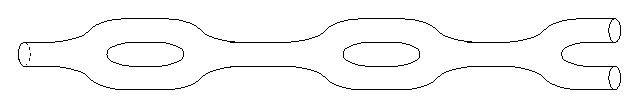
\includegraphics{cob2.eps}}
\cell{-1}{26}{bl}{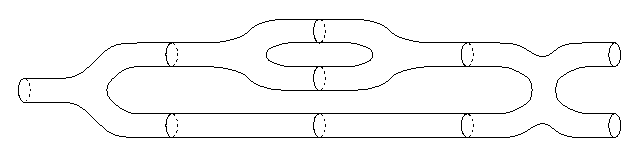
\includegraphics{cob1.eps}}
% arrows
\put(0,30){\vector(0,-1){20}}
\cell{2}{19}{l}{\cong}
\put(100,24){\vector(0,-1){10}}
\cell{98}{19}{r}{\cong}
\cell{49}{19}{l}{\Downarrow\ \cong}
\end{picture}
% \end{array}
% \]
% \hand{55}{15}
\caption{2-cell in the \fc-multicategory $1\hyph\fcat{Mfd}_2$, with 4
horizontal 1-cells along the top row}
\label{fig:cobordisms}
\end{figure}
%
shows a 2-cell in the underlying \fc-multicategory of $1\hyph\fcat{Mfd}_2$,
in a case where all the continuous maps involved are homeomorphisms.

Similar constructions can be made for other types of manifold: oriented,
smooth, holomorphic, \ldots.  There is a slight problem with identities for
horizontal composition, as the horizontal identity on $A$ `ought' to be
just $A$ itself (compare~\ref{eg:wk-dbl-cospan}) but this is not usually
counted as an $(n+1)$-manifold with boundary.  Whether or not we can fix
this, there is certainly an underlying $\fc$-multicategory: the problem is
purely one of representability.
\end{example}





\section{Monads, monoids and modules}
\lbl{sec:mmm}


Modules have loomed large in our examples of \fc-multicategories, appearing
as horizontal 1-cells.  Monoids and their cousins (such as rings and
categories) have also been prominent, appearing as 0-cells.  Here we show
how any \fc-multicategory $C$ gives rise to a new \fc-multicategory
$\Mon(C)$, whose 0-cells are monoids/monads in $C$ and whose horizontal
1-cells are modules between them.  

As I shall explain, this construction has traditionally been carried out in
a narrower context than \fc-multicategories, which has meant working under
certain technical restrictions.  If we expand to the wider context of
\fc-multicategories then the technicalities vanish.  

For an example of the traditional construction, start with the monoidal
category $(\Ab, \otimes, \integers)$ of abelian groups.  A monoid therein
is just a ring.  Given two monoids $A$, $B$ in a monoidal category, a
\demph{$(B,A)$-module}%
%
\index{module!monoids@over monoids}
%
is an object $M$ equipped with compatible left and
right actions
\[
B \otimes M \goby{\act{\mi{L}}} M,
\diagspace
M \otimes A \goby{\act{\mi{R}}} M,
\]
and there is an obvious notion of map between $(B,A)$-modules.  In this
particular case these are (bi)modules and their homomorphisms, in the usual
sense.  So we have almost arrived at the bicategory of~\ref{eg:bicat-Ring}:
0-cells are rings, 1-cells are modules, and 2-cells are maps of modules.
The only missing ingredient is the tensor product of modules.  If $M$ is a
$(B,A)$-module and $N$ a $(C,B)$-module then $N \otimes_B M$ is a quotient
of the abelian group tensor $N\otimes M$; categorically, it is the
(reflexive) coequalizer%
%
\index{coequalizer}
%
\[
\begin{diagram}[scriptlabels]
N \otimes B \otimes M	&
\pile{	\rTo^{\act{\mi{R}} \otimes 1_M}\\
	\rTo_{1_N \otimes \act{\mi{L}}} }	&
N\otimes M	&
\rTo	&
N \otimes_B M.	\\
\end{diagram}
\]
The abelian group $N\otimes M$ acquires a $(C,A)$-module structure just as
long as the endofunctors $C\otimes \dashbk$ and $\dashbk\otimes A$ of $\Ab$
preserve (reflexive) coequalizers, which they do.  The rest of the
bicategory structure comes easily.  So from the monoidal category $(\Ab,
\otimes, \integers)$ we have derived the bicategory of rings, modules and
maps of modules.  

In the same way, any monoidal category $(\cat{A}, \otimes, I)$ gives rise
to a bicategory $\Mon(\cat{A})$ of monoids and modules in $\cat{A}$, as
long as $\cat{A}$ has reflexive coequalizers and these are preserved by the
functors $A \otimes \dashbk$ and $\dashbk \otimes A$ for all $A \in
\cat{A}$.  Generalizing, any bicategory $\cat{B}$ gives rise to a
bicategory $\Mon(\cat{B})$ of monads and modules in $\cat{B}$, as long as
$\cat{B}$ locally has reflexive coequalizers and these are preserved by the
functors $f\of\dashbk$ and $\dashbk\of f$ for all 1-cells $f$.

There are two unsatisfactory aspects to this construction.  One is the
necessity of the coequalizer conditions.  The other is that homomorphisms
of monoids are conspicuous by their absence: for instance, ring
homomorphisms are not an explicit part of $\Mon(\Ab)$ (although they can be
recovered as those 1-cells of $\Mon(\Ab)$ that have a right adjoint).  The
following definition for \fc-multicategories solves both problems.

\begin{defn}
Let $C$ be an \fc-multicategory. The \fc-multicategory $\Mon(C)$%
% 
\glo{fcmtiMon}%
%
\index{monads construction}
%
% 
is defined as
follows.
%
\begin{itemize}
%
\item
A 0-cell of $\Mon(C)$ is an \fc-multicategory map $1\go C$.  That is, it is
a 0-cell $a$ of $C$ together with a horizontal 1-cell $a\goby{t}a$ and
2-cells
\[
\begin{fcdiagram}
a	&\rTo^{t}	&a			&\rTo^{t}	&a	\\
\dTo<{1}&		&\Downarrow\tcs{\mu}	&		&\dTo>{1}\\
a	&		&\rTo_{t}		&		&a	\\
\end{fcdiagram}
\diagspace
\begin{fcdiagram}
a	&\rEquals		&a	\\
\dTo<{1}&\Downarrow\tcs{\eta}	&\dTo>{1}\\
a	&\rTo_{t}		&a	\\
\end{fcdiagram}
\]
satisfying the usual axioms for a monad, $\mu\of\pr{\mu}{1_t} =
\mu\of\pr{1_t}{\mu}$ and $\mu\of\pr{\eta}{1_t} = 1_t = \mu\of\pr{1_t}{\eta}$.

\item
A vertical 1-cell
\[
\begin{fcdiagram}
(a,t,\mu,\eta)	\\
\dTo		\\
(\hat{a},\hat{t},\hat{\mu},\hat{\eta})\\
\end{fcdiagram}
\]
in $\Mon(C)$ is a vertical 1-cell
\[
\begin{fcdiagram}
a	\\
\dTo>f	\\
\hat{a}	\\
\end{fcdiagram}
\]
in $C$ together with a 2-cell
\[
\begin{fcdiagram}
a		&\rTo^{t}		&a		\\
\dTo<{f}	&\Downarrow\tcs{\omega}	&\dTo>{f}	\\
\hat{a}		&\rTo_{\hat{t}}		&\hat{a}	\\
\end{fcdiagram}
\]
such that $\omega\of\mu = \hat{\mu}\of\pr{\omega}{\omega}$ and
$\omega\of\eta = \hat{\eta}\of f$.  (The notation $\hat{\eta} \of f$ is
explained on p.~\pageref{p:null-notation}.)

\item
A horizontal 1-cell $(a,t,\mu,\eta) \rTo (a',t',\mu',\eta')$ is a
horizontal 1-cell $a\goby{m}a'$ in $C$ together with 2-cells
\[
\begin{fcdiagram}
a	&\rTo^{t}	&a			&\rTo^{m}	&a'	\\
\dTo<{1}&		&\Downarrow\tcs{\chi}	&		&\dTo>{1}\\
a	&		&\rTo_{m}		&		&a'	\\
\end{fcdiagram}
\diagspace
\begin{fcdiagram}
a	&\rTo^{m}	&a'			&\rTo^{t'}	&a'	\\
\dTo<{1}&		&\Downarrow\tcs{\chi'}	&		&\dTo>{1}\\
a	&		&\rTo_{m}		&		&a'	\\
\end{fcdiagram}
\]
satisfying the usual module axioms, $\chi\of\pr{\mu}{1_m} =
\chi\of\pr{1_t}{\chi}$, $\chi\of\pr{\eta}{1_m}=1_m$, and dually for
$\chi'$, and the `commuting actions' axiom, $\chi'\of\pr{\chi}{1_{t'}} =
\chi\of\pr{1_t}{\chi'}$.

\item
A 2-cell
\[
\begin{fcdiagram}
t_0	&\rTo^{m_1}	&t_1	&\rTo^{m_2}	&\ 	&\cdots	
&\ 	&\rTo^{m_{n}}	&t_n	\\
\dTo<{f}&		&	&		&\Downarrow	&	
&	&		&\dTo>{f'}\\
t	&		&	&		&\rTo_{m}	&	
&	&		&t'	\\
\end{fcdiagram}
\]
in $\Mon(C)$, where $t$ stands for $(a,t,\mu,\eta)$, $m$ for
$(m, \chi, \chi')$, $f$ for \pr{f}{\omega}, and so on, is a 2-cell
\[
\begin{fcdiagram}
a_0	&\rTo^{m_1}	&a_1	&\rTo^{m_2}	&\ 	&\cdots	
&\ 	&\rTo^{m_{n}}	&a_n	\\
\dTo<{f}&		&	&		&\Downarrow\tcs{\theta}&	
&	&		&\dTo>{f'}\\
a	&		&	&		&\rTo_{m}	&	
&	&		&a'	\\
\end{fcdiagram}
\]
in $C$ satisfying the `external equivariance' axioms
%
\begin{eqnarray*}
\theta\of(\chi_1,\range{1_{m_2}}{1_{m_n}}) 		&=&
\chi\of\pr{\omega}{\theta}				\\
\theta\of(\range{1_{m_1}}{1_{m_{n-1}}},\chi'_n)	&=&
\chi'\of\pr{\theta}{\omega'}
\end{eqnarray*}
%
and the `internal equivariance' axioms
%
\begin{eqnarray*}
\lefteqn{\theta\of(\range{1_{m_1}}{1_{m_{i-2}}}, \chi'_{i-1}, 1_{m_{i}},
\range{1_{m_{i+1}}}{1_{m_n}})		=}				\\
&&\theta\of(\range{1_{m_1}}{1_{m_{i-2}}}, 1_{m_{i-1}}, \chi_i,
\range{1_{m_{i+1}}}{1_{m_n}}) 
\end{eqnarray*}
%
for $2\leq i\leq n$.

\item
Composition and identities for both 2-cells and vertical 1-cells in
$\Mon(C)$ are just composition and identities in $C$.
\end{itemize}
%
\end{defn}
%
With the obvious definition on maps of \fc-multicategories, this gives a
functor 
\[
\Mon: \fc\hyph\Multicat \go \fc\hyph\Multicat.
\]

\begin{example}%
%
\index{double category!weak!bicategory@\vs.\ bicategory}%
%
\index{bicategory!weak double category@\vs.\ weak double category}
%
Our new $\Mon$ generalizes the traditional $\Mon$ in the following sense.
Let $B$ be a bicategory satisfying the conditions on local reflexive
coequalizers mentioned above, so that it is possible to construct the
bicategory $\Mon(B)$ in the traditional way.  Let $C$ be the
\fc-multicategory corresponding to $B$ (Example~\ref{eg:fcm-bicat}), with
only trivial vertical 1-cells.  Then a 0-cell of $\Mon(C)$ is a monad in
$B$, a horizontal 1-cell $t \go t'$ is a $(t',t)$-module in $B$, and a
2-cell of the form 
\[
\begin{fcdiagram}
t_0	&\rTo^{m_1}	&t_1	&\rTo^{m_2}	&\ 	&\cdots	
&\ 	&\rTo^{m_{n}}	&t_n	\\
\dTo<1	&		&	&		&\Downarrow	&	
&	&		&\dTo>1	\\
t_0	&		&	&		&\rTo_m		&	
&	&		&t_n	\\
\end{fcdiagram}
\]
is a map
\[
m_n \otimes_{t_{n-1}} \cdots 
\otimes_{t_2} m_2 \otimes_{t_1} m_1
\go
m
\]
of $(t_n, t_0)$-modules---that is, a 2-cell in $\Mon(B)$.  So if we discard
the non-identity vertical 1-cells of $\Mon(C)$ then we obtain the
\fc-multicategory corresponding to $\Mon(B)$.
\end{example}

\begin{example}%
%
\index{fc-multicategory@$\fc$-multicategory!rings@of rings}
%
Take the monoidal category $(\Ab,\otimes,\integers)$ and the corresponding
\fc-multicategory $\Sigma\Ab$ (Example~\ref{eg:fcm-mon-cat}).  Then
$\Mon(\Sigma\Ab)$ is $\fcat{Ring}_2$, the \fc-multicategory of
Example~\ref{eg:fcm-Ring} in which 0-cells are rings, vertical 1-cells are
homomorphisms of rings, horizontal 1-cells are modules%
%
\index{module!bimodule over rings}
%
between rings, and
2-cells are module maps of a suitable kind.  
\end{example}

\begin{example}%
%
\index{fc-multicategory@$\fc$-multicategory!monoids@of monoids}
%
Similarly, if we take the monoidal category $(\Set,\times,1)$ then
$\Mon(\Sigma\Set)$ is (the underlying \fc-multicategory of) the weak double
category $\fcat{Monoid}_2$ (Example~\ref{eg:wk-dbl-Monoid}).
\end{example}

\begin{example}
Take the \fc-multicategory $\Set_2$ of sets, functions and
spans~(\ref{eg:fcm-wk-dbl}).  Then a 0-cell of $\Mon(\Set_2)$ is a monad in
$\Set_2$, that is, a small category.%
%
\index{fc-multicategory@$\fc$-multicategory!categories@of categories}%
%
\index{double category!weak!categories@of categories}%
%
\index{category!weak double category of}
%
 A vertical 1-cell is a functor; a
horizontal 1-cell is a module.  A 2-cell
\[
\begin{fcdiagram}
A_0	&\rTo^{M_1}	&A_1	&\rTo^{M_2}	&\ 	&\cdots	
&\ 	&\rTo^{M_n}	&A_n	\\
\dTo<F	&		&	&		&\Downarrow\tcs{\theta}&
&	&		&\dTo>{F'}\\
A	&		&	&		&\rTo_{M}	&	
&	&		&A'	\\
\end{fcdiagram}
\]
consists of a function
\[
\theta_{a_0, \ldots, a_n}: 
M_n(a_{n-1}, a_n) \times\cdots\times M_1(a_0, a_1) 
\go
M(Fa_0, F'a_n)
\]
for each $a_0 \in A_0, \ldots, a_n \in A_n$, such that this family is
natural in the $a_i$'s.  So $\Mon(\Set_2)$ is $\Cat_2$, the weak double
category of~\ref{eg:wk-dbl-Cat}.
\end{example}

This last example leads us to definitions of module and transformation for
generalized multicategories.  Let $T$ be a cartesian monad on a cartesian
category $\Eee$.  Recall the \fc-multicategory $\Sp{\Eee}{T}$
of~\ref{eg:wk-dbl-T-span}, and consider the \fc-multicategory
$\Mon(\Sp{\Eee}{T})$.  A 0-cell of $\Mon(\Sp{\Eee}{T})$ is a monad in
$\Sp{\Eee}{T}$, that is, a $T$-multicategory, so we write $T\hyph\Multicat$
for $\Mon(\Sp{\Eee}{T})$.  A vertical 1-cell is a map of
$T$-multicategories.  A horizontal 1-cell $A \go B$ will be called a
\demph{$(B,A)$-module}.%
%
\index{module!generalized multicategories@over generalized multicategories}%
%
\index{generalized multicategory!module over}
%
%
 To see what modules are explicitly, note that the
underlying graph
\[
\begin{slopeydiag}
	&	&B_1	&	&	\\
	&\ldTo<\dom&	&\rdTo>\cod&	\\
TB_0	&	&	&	&B_0	\\
\end{slopeydiag}
\]
of $B$ is a horizontal 1-cell in $\Sp{\Eee}{T}$, composition with which
defines an endofunctor $B\of\dashbk$ of the category $\Sp{\Eee}{T} (A_0,
B_0)$ of diagrams of the form  
%
\begin{equation}	\label{diag:module-span}
\begin{slopeydiag}
	&	&M	&	&	\\
	&\ldTo	&	&\rdTo	&	\\
TA_0	&	&	&	&B_0.	\\
\end{slopeydiag}
\end{equation}
%
Moreover, the multicategory structure of $B$ gives $B\of\dashbk$ the
structure of a monad on $\Sp{\Eee}{T} (A_0, B_0)$.  Dually, the
multicategory $A$ also induces a monad $\dashbk\of A$ on $\Sp{\Eee}{T}
(A_0, B_0)$, and there is a canonical isomorphism $(B\of\dashbk)\of A \iso
B\of(\dashbk\of A)$ compatible with the monad structures (formally, a
distributive law:~\ref{defn:distrib-law}).  So a $(B,A)$-module is a
diagram~\bref{diag:module-span} in $\Eee$ together with maps $\act{\mi{L}}:
B \of M \go M$ and $\act{\mi{R}}: M \of A \go M$ such that
$(M,\act{\mi{L}})$ and $(M,\act{\mi{R}})$ are algebras for the monads
$B\of\dashbk$ and $\dashbk\of A$ respectively, and the following diagram
commutes:
\[
\begin{diagram}[size=2em,scriptlabels]
	&(B\of M)\of A 	&\iso 	&B\of (M\of A)	&	\\
\ldTo(1,2)<{\act{\mi{L}}*1_A}&&	&		&
\rdTo(1,2)>{1_B * \act{\mi{R}}}\\
M\of A	&		&	&		&B\of M	\\
	&\rdTo<{\act{\mi{R}}}&	&\ldTo>{\act{\mi{L}}}&	\\
	&		&M.	&		&	\\
\end{diagram}
\]

This definition generalizes the definition for plain
multicategories~(\ref{sec:om-further}).  Just as there, it also makes sense
to define left and right modules for a $T$-multicategory: do not take a
whole span $M$, but only the right-hand or left-hand half.  A \demph{left
$B$-module} is nothing other than a $B$-algebra.  A \demph{right $A$-module}
(or \demph{$A$-coalgebra})%
%
\index{coalgebra}
%
is an object $M$ of $\Eee/TA_0$ (thought of as a
span
\[
\begin{slopeydiag}
	&	&M	&	&	\\
	&\ldTo	&	&\rdGet	&	\\
TA_0	&	&	&	&\cdot	\\
\end{slopeydiag}
\]
with a phantom right leg) together with a map $h: M\of A \go M$ making $M$
into an algebra for the monad $\dashbk\of A$ on $\Eee/TA_0$.  

In general, $T\hyph\Multicat$ is not a weak double category: there is no
tensor%
%
\index{tensor!generalized multicategory@over generalized multicategory}
%
product of modules.  For to tensor modules we would need $\Eee$ to
possess reflexive coequalizers and $T$ to preserve them, and although the
requirement on $\Eee$ is satisfied in almost all of the examples that we
consider, the requirement on $T$ is not---for instance, when $T=\fc$.

There is, however, an `identity' horizontal 1-cell on each object.  Given a
$T$-multicategory $A$, this is the $(A,A)$-module $I_A$ whose underlying
span is
\[
\begin{slopeydiag}
	&	&A_1	&	&	\\
	&\ldTo<\dom&	&\rdTo>\cod&	\\
TA_0	&	&	&	&A_0	\\
\end{slopeydiag}
\]
and whose actions are both composition in $A$.  Recalling the remarks on
natural transformations in Example~\ref{eg:wk-dbl-Cat}, we make the
following definition.  Let $A \parpair{f}{f'} B$ be maps of
$T$-multicategories.  A \demph{transformation}%
%
\index{transformation!generalized multicategories@of generalized multicategories}%
%
\index{generalized multicategory!transformation of}
%
\begin{equation}	\label{diag:T-transf}
A 
\ctwomult{\scriptstyle f}{\scriptstyle f'}{\scriptstyle \alpha} 
B
\end{equation}
%
of $T$-multicategories is a 2-cell 
\[
\begin{fcdiagram}
A	&\rTo^{I_A}		&A	\\
\dTo<f	&\Downarrow\tcs{\alpha}	&\dTo>{f'}\\
B	&\rTo_{I_B}		&B
\end{fcdiagram}
\]
in $T\hyph\Multicat$.  Explicitly, a transformation $f \go f'$ is a map
$\alpha: A_1 \go B_1$ such that the diagrams 
%
\begin{equation}	\label{eqs:T-transf}
\begin{slopeydiag}
	&		&A_1	&		&	\\
	&\ldTo^\dom	&	&\rdTo^\cod	&	\\
TA_0	&		&\dTo>\alpha&		&A_0	\\
\dTo<{Tf_0}&		&B_1	&		&\dTo>{f'_0}\\
	&\ldTo^\dom	&	&\rdTo^\cod	&	\\
TB_0	&		&	&		&B_0	\\
\end{slopeydiag}
%
\diagspace
\diagspace
%
% \begin{slopeydiag}
\begin{diagram}[size=2em,scriptlabels]
	&		&A_1\of A_1	&		&	\\
	&\ldTo<{\alpha*f_1}&\dTo~\comp	&\rdTo>{f'_1*\alpha}&	\\
B_1\of B_1&		&A_1		&		&B_1\of B_1\\
	&\rdTo<\comp	&\dTo~\alpha	&\ldTo>\comp	&	\\
	&		&B_1		&		&	\\
\end{diagram}
% \end{slopeydiag}
\end{equation}
%
commute, where the map $\alpha * f_1: A_1 \of A_1 \go B_1\of B_1$ is
induced by the maps $\alpha: A_1 \go B_1$ and $f_1: A_1 \go B_1$,
% via the definitions of $A_1 \of A_1$ and $B_1 \of B_1$ as pullbacks, 
and similarly $f'_1 * \alpha$.

This may come as a surprise: if $A$ and $B$ are ordinary categories and
$\alpha$ a natural transformation as in~\bref{diag:T-transf} then we would
usually think of $\alpha$ as a map $A_0 \go B_1$, not $A_1 \go B_1$.
Observe, however, that $\alpha$ assigns to each map $a \goby{\theta} a'$ in
$A$ a map $fa \goby{\alpha_\theta} f'a'$ in $B$, the diagonal of the
naturality square for $\alpha$ at $\theta$.  Since $\alpha_a$ can be
recovered as $\alpha_{1_a}$ for each $a\in A$, it must be possible to
define a natural transformation~\bref{diag:T-transf} as a map $A_1 \go B_1$
satisfying axioms.  The same goes for transformations of plain
multicategories, where now $\alpha_\theta$ is either side of the equation
in Fig.~\ref{fig:cl-transf-axiom} (p.~\pageref{fig:cl-transf-axiom}).  For
generalized multicategories we also have the choice between viewing
transformations as maps $A_0 \go B_1$ or as maps $A_1 \go B_1$; the axioms
for the $A_0 \go B_1$ version can easily be worked out (or looked up:
Leinster \cite[1.1.1]{GECM}).  

For general cartesian $T$, suppose that we discard from the
\fc-multicategory $T\hyph\Multicat$ all of the horizontal 1-cells except
for the `identities' (those of the form $I_A$).  Then we obtain a weak
double category whose only horizontal 1-cells are identities---in other
words~(\ref{eg:wk-dbl-degen}), a strict 2-category.  Concretely:
transformations can be composed vertically and horizontally, and this makes
$T\hyph\Multicat$%
% 
\glo{TMulticat2cat}
% 
into a strict 2-category.





\begin{notes}

Many \fc-multicategories are weak double categories.  Many
\fc-multicategories also have the property that every vertical 1-cell
$f: a \go b$ gives rise canonically to cells
\[
\begin{fcdiagram}
a	&\rEquals	&a	\\
\dTo<1	&\Downarrow	&\dTo>f	\\
a	&\rTo		&b\makebox[0em][l]{,}	\\	
\end{fcdiagram}
% 
\diagspace
% 
\begin{fcdiagram}
a	&\rEquals	&a	\\
\dTo<f	&\Downarrow	&\dTo>1	\\
b	&\rTo		&a
\end{fcdiagram}
\]
(as is familiar in $\fcat{Ring}_2$, for instance).  These two properties
combine to say that any diagram
\[
\begin{fcdiagram}
a_0	&\rTo^{m_1}	&a_1	&\rTo^{m_2}	&\ 	&\cdots	
&\ 	&\rTo^{m_n}	&a_n	\\
\dTo<{f}&		&	&		&	&
&	&		&\dTo>{f'}\\
a	&		&	&		&	&	
&	&		&a'	\\
\end{fcdiagram}
\]
has a 2-cell filling it in (canonically, up to isomorphism): the weak
double category structure provides a fill-in when $f$ and $f'$ are both
identities, the vertical-to-horizontal property provides a fill-in when
$n=0$ and one of $f$ or $f'$ is an identity, and the general case can be
built up from these special cases.  The exact situation is still unclear,
but there are obvious similarities between this, the representations of
plain multicategories in~\ref{sec:non-alg-notions}, and the universal
opetopic cells in~\ref{sec:ope-n}.

The $\fc$-multicategory $\Set[V]$ of~\ref{eg:fcm-matrices} appears in a
different guise in Carboni,%
%
\index{Carboni, Aurelio}
%
Kasangian%
%
\index{Kasangian, Stefano}
%
and Walters~\cite{CKW},%
%
\index{Walters, Robert}
%
under the
name of `matrices'.%
%
\index{matrix}
%
 Weak double categories have also been studied by
Grandis%
%
\index{Grandis, Marco}
%
and Par\'e~\cite{GPLDC, GPADC}.%
%
\index{Pare, Robert@Par\'e, Robert}
%
 


\end{notes}
